\documentclass{standalone}
\usepackage[T1]{fontenc}
\usepackage[utf8]{inputenc}
\usepackage[usenames,dvipsnames]{xcolor}
\usepackage{tikz}
\usetikzlibrary{plotmarks}
\usetikzlibrary{shapes,snakes,arrows}
\begin{document}
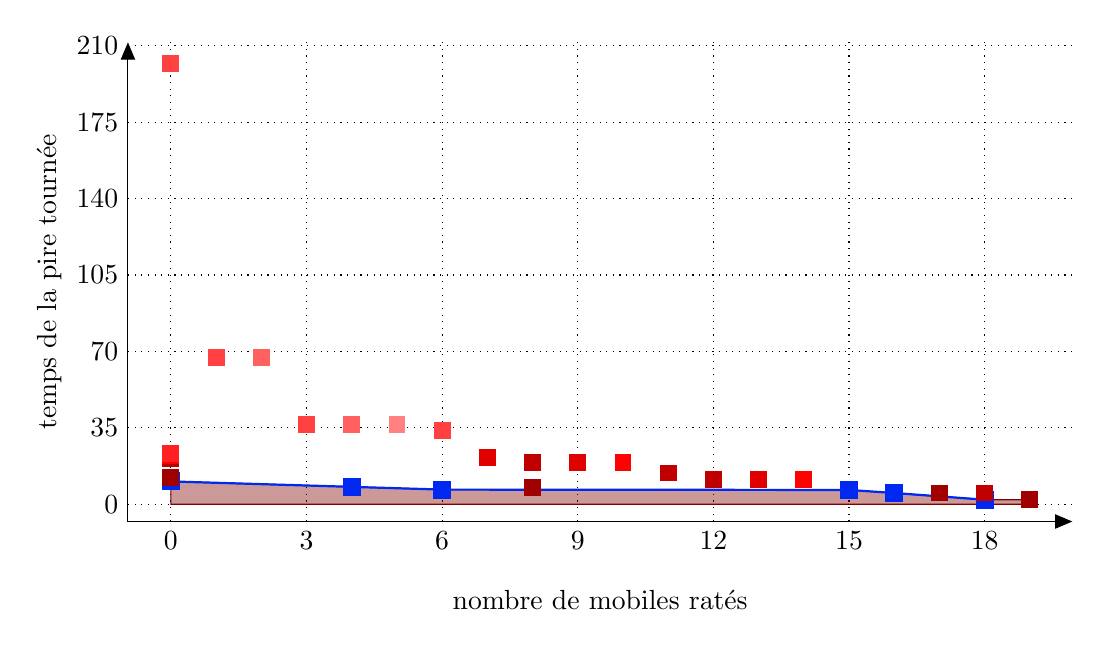
\begin{tikzpicture}[xscale=0.574163,yscale=0.0277214]
\draw[xstep=3,ystep=35,thin,dotted,color=Black] (-0.95,-7.89917) grid (19.9383,211.55);
\begin{scope}
  \clip (-0.95,-7.89917) rectangle (19.9383,211.55);
  \definecolor{hvColor}{RGB}{128,0,0}
  \draw[color=hvColor, fill=hvColor, fill opacity=0.4] (0,2.08765) -- (0,10.4594) -- (4,7.97055) -- (6,6.71603) -- (15,6.55359) -- (16,5.14916) -- (18,2.08765) -| (19,2.08765) |- (0,0) -- cycle;
  \definecolor{pLineColor}{RGB}{128,0,0}
  \definecolor{pPointColor}{RGB}{0,40,240}
  \draw[thick,color=pPointColor] (0,10.4594) node[draw,color=pPointColor,fill=pPointColor, inner sep = 0pt, minimum size=2mm] {} -- (4,7.97055) node[draw,color=pPointColor,fill=pPointColor, inner sep = 0pt, minimum size=2mm] {} -- (6,6.71603) node[draw,color=pPointColor,fill=pPointColor, inner sep = 0pt, minimum size=2mm] {} -- (15,6.55359) node[draw,color=pPointColor,fill=pPointColor, inner sep = 0pt, minimum size=2mm] {} -- (16,5.14916) node[draw,color=pPointColor,fill=pPointColor, inner sep = 0pt, minimum size=2mm] {} -- (18,2.08765) node[draw,color=pPointColor,fill=pPointColor, inner sep = 0pt, minimum size=2mm] {};

  \definecolor{pLineColor}{RGB}{160,0,0}
  \definecolor{pPointColor}{RGB}{160,0,0}
  \node [draw,color=pPointColor,fill=pPointColor, inner sep = 0pt, minimum size=2mm] at (0,12.2265) {};
  \node [draw,color=pPointColor,fill=pPointColor, inner sep = 0pt, minimum size=2mm] at (8,7.51176) {};
  \node [draw,color=pPointColor,fill=pPointColor, inner sep = 0pt, minimum size=2mm] at (17,5.14916) {};
  \node [draw,color=pPointColor,fill=pPointColor, inner sep = 0pt, minimum size=2mm] at (19,2.08765) {};
  \definecolor{pLineColor}{RGB}{192,0,0}
  \definecolor{pPointColor}{RGB}{192,0,0}
  \node [draw,color=pPointColor,fill=pPointColor, inner sep = 0pt, minimum size=2mm] at (0,21.0649) {};
  \node [draw,color=pPointColor,fill=pPointColor, inner sep = 0pt, minimum size=2mm] at (8,19.2932) {};
  \node [draw,color=pPointColor,fill=pPointColor, inner sep = 0pt, minimum size=2mm] at (11,14.3302) {};
  \node [draw,color=pPointColor,fill=pPointColor, inner sep = 0pt, minimum size=2mm] at (12,11.2603) {};
  \node [draw,color=pPointColor,fill=pPointColor, inner sep = 0pt, minimum size=2mm] at (18,5.14916) {};
  \definecolor{pLineColor}{RGB}{224,0,0}
  \definecolor{pPointColor}{RGB}{224,0,0}
  \node [draw,color=pPointColor,fill=pPointColor, inner sep = 0pt, minimum size=2mm] at (0,22.1747) {};
  \node [draw,color=pPointColor,fill=pPointColor, inner sep = 0pt, minimum size=2mm] at (7,21.5963) {};
  \node [draw,color=pPointColor,fill=pPointColor, inner sep = 0pt, minimum size=2mm] at (9,19.2932) {};
  \node [draw,color=pPointColor,fill=pPointColor, inner sep = 0pt, minimum size=2mm] at (13,11.2603) {};
  \definecolor{pLineColor}{RGB}{255,1,1}
  \definecolor{pPointColor}{RGB}{255,1,1}
  \node [draw,color=pPointColor,fill=pPointColor, inner sep = 0pt, minimum size=2mm] at (0,22.4093) {};
  \node [draw,color=pPointColor,fill=pPointColor, inner sep = 0pt, minimum size=2mm] at (10,19.2932) {};
  \node [draw,color=pPointColor,fill=pPointColor, inner sep = 0pt, minimum size=2mm] at (14,11.2603) {};
  \definecolor{pLineColor}{RGB}{255,33,33}
  \definecolor{pPointColor}{RGB}{255,33,33}
  \node [draw,color=pPointColor,fill=pPointColor, inner sep = 0pt, minimum size=2mm] at (0,23.4044) {};
  \definecolor{pLineColor}{RGB}{255,65,65}
  \definecolor{pPointColor}{RGB}{255,65,65}
  \node [draw,color=pPointColor,fill=pPointColor, inner sep = 0pt, minimum size=2mm] at (0,201.824) {};
  \node [draw,color=pPointColor,fill=pPointColor, inner sep = 0pt, minimum size=2mm] at (1,67.1062) {};
  \node [draw,color=pPointColor,fill=pPointColor, inner sep = 0pt, minimum size=2mm] at (3,36.5789) {};
  \node [draw,color=pPointColor,fill=pPointColor, inner sep = 0pt, minimum size=2mm] at (6,33.6687) {};
  \definecolor{pLineColor}{RGB}{255,97,97}
  \definecolor{pPointColor}{RGB}{255,97,97}
  \node [draw,color=pPointColor,fill=pPointColor, inner sep = 0pt, minimum size=2mm] at (2,67.1062) {};
  \node [draw,color=pPointColor,fill=pPointColor, inner sep = 0pt, minimum size=2mm] at (4,36.5789) {};
  \definecolor{pLineColor}{RGB}{255,129,129}
  \definecolor{pPointColor}{RGB}{255,129,129}
  \node [draw,color=pPointColor,fill=pPointColor, inner sep = 0pt, minimum size=2mm] at (5,36.5789) {};
\end{scope}
\draw[->,>=triangle 45] (-0.95,-7.89917) -- coordinate (x axis mid) (19.9383,-7.89917);
\node[below=1cm,anchor=center] at (x axis mid) {nombre de mobiles ratés};
\foreach \x in {0,3,6,9,12,15,18}
  \draw (\x,-7.89917) -- (\x,-7.89917) node[anchor=north] {\x};
\draw[->,>=triangle 45] (-0.95,-7.89917) -- coordinate (y axis mid) (-0.95,211.55);
\node[left=1cm,rotate=90,anchor=center] at (y axis mid) {temps de la pire tournée};
\foreach \y in {0,35,70,105,140,175,210}
  \draw (-0.95,\y) -- (-0.95,\y) node[anchor=east] {\y};
\end{tikzpicture}
\end{document}
